% \documentclass{standalone}
% \usepackage{currfile,hyperxmp}

% \input{../tikz_header.tex}

% \begin{document}



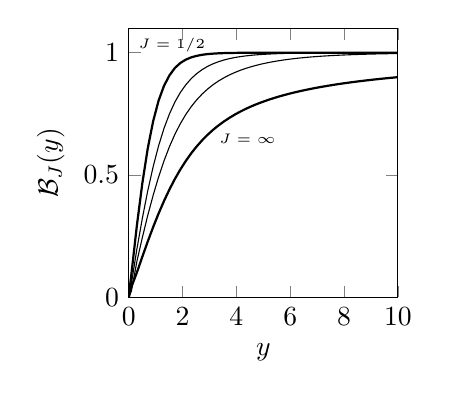
\begin{tikzpicture}[
    declare function={coth(\x)  = 1/tanh(\x) ; 
    af(\J) = (2*\J +1 )/(2*\J);
    bf(\J) = 1/(2*\J);
                 },
]
%\useasboundingbox (-1.3,-1.2) rectangle (10.2,4.7);
%\draw (-1,-1) rectangle +(12,5);

    \begin{axis}[ xlabel={ $y$ }, ylabel= {$\mathcal{B}_J(y)$}, 
         width=50mm, height=50mm, 
        %ymode=log, 
     %   ymode=log,
         xmin = 0,
         xmax = 10,
         ymin = 0,
     %    ymin  = 0,
      %   ymax = 2.1,
         %xmax=5.5, ymin = 0, ymax=7.5,
        % axis x line=bottom,
        % axis y line=left,
         % xmax= 2e5, unbounded coords=jump, ymin=0, ymax = 4
        % label style={font=\tiny},
        % tick label style={font=\tiny}
      %  ytick= \empty ,
      %  xtick= \empty, 
     %  legend pos= north west,
     %  legend style={draw=none, font=\footnotesize}
     %clip = false,
    ]




    \addplot[domain=-10:10 , samples=100 ]{ af(1) * coth(af(1) * x) - bf(1) * coth(bf(1) * x) };
    \addplot[domain=-10:10 , samples=100, thick]{ af(0.5) * coth(af(0.5) * x) - bf(0.5) * coth(bf(0.5) * x) };
    \addplot[domain=-10:10 , samples=100 ]{ af(2) * coth(af(2) * x) - bf(2) * coth(bf(2) * x) };
   \addplot[domain=-10:10 , samples=100, thick ]{ coth( x) - 1 / x };
 
   \node[right, font=\tiny] at (0,1.03) { $J = 1/2$};
   \node[right, font=\tiny] at (3,0.65) { $J = \infty$};

   %\draw[thin](-10,0) --(10,0);
   %\draw[thin](0,-10) --(0,10);
   

    \end{axis}
\end{tikzpicture}

%\end{document}